\documentclass[11pt,letterpaper]{article}
\usepackage[margin=1in]{geometry}
\usepackage{graphicx}
\usepackage{hyperref}
\usepackage{enumitem}
\usepackage{amsmath}
\usepackage{amsfonts}
\usepackage{booktabs}
\usepackage{xcolor}
\usepackage{fancyhdr}
\usepackage{titlesec}
\usepackage{url}
\usepackage{float}

% Configure hyperlinks
\hypersetup{
    colorlinks=true,
    linkcolor=blue,
    urlcolor=blue,
    citecolor=blue
}

% Configure headers
\pagestyle{fancy}
\fancyhf{}
\rhead{Jiang | Immigrants Against Immigrants?}
\lhead{ASA 2025}
\cfoot{\thepage}

% Configure section formatting
\titleformat{\section}{\Large\bfseries}{\thesection}{1em}{}
\titleformat{\subsection}{\large\bfseries}{\thesubsection}{1em}{}
\titleformat{\subsubsection}{\normalsize\bfseries}{\thesubsubsection}{1em}{}

% CUSTOM SMALLER BULLETS
% Define smaller bullet symbols
\newcommand{\smallbullet}{\raisebox{0.25ex}{\scalebox{0.6}{$\bullet$}}}
\newcommand{\smalldash}{\raisebox{0.1ex}{\scalebox{0.8}{--}}}
\newcommand{\smallcirc}{\raisebox{0.25ex}{\scalebox{0.6}{$\circ$}}}
\newcommand{\smalldot}{\raisebox{0.25ex}{\scalebox{0.5}{$\cdot$}}}

% CUSTOMIZABLE INDENTATION SYSTEM
% Define your indentation step size here:
\newlength{\indentStep}
\setlength{\indentStep}{1.5em}  % Change this value to adjust indentation spacing

% Calculate indentations automatically
\newlength{\levelOneIndent}
\newlength{\levelTwoIndent}
\newlength{\levelThreeIndent}
\newlength{\levelFourIndent}

\setlength{\levelOneIndent}{2\indentStep}      % 3.0em with 1.5em step
\setlength{\levelTwoIndent}{3.5\indentStep}    % 5.25em with 1.5em step
\setlength{\levelThreeIndent}{4.5\indentStep}  % 6.75em with 1.5em step
\setlength{\levelFourIndent}{5.5\indentStep}   % 8.25em with 1.5em step

% Apply the calculated indentations with smaller bullets
\setlist[itemize,1]{
    leftmargin=\levelOneIndent,
    labelsep=1em,
    itemindent=0pt,
    label=\smallbullet,
    itemsep=2pt,
    parsep=0pt,
    topsep=3pt
}
\setlist[itemize,2]{
    leftmargin=\levelTwoIndent,
    labelsep=1em,
    itemindent=0pt,
    label=\smalldash,
    itemsep=1pt,
    parsep=0pt,
    topsep=2pt
}
\setlist[itemize,3]{
    leftmargin=\levelThreeIndent,
    labelsep=1em,
    itemindent=0pt,
    label=\smallcirc,
    itemsep=1pt,
    parsep=0pt,
    topsep=2pt
}
\setlist[itemize,4]{
    leftmargin=\levelFourIndent,
    labelsep=1em,
    itemindent=0pt,
    label=\smalldot,
    itemsep=1pt,
    parsep=0pt,
    topsep=2pt
}

% Enumerate with slightly more space for numbers
\setlist[enumerate,1]{
    leftmargin=\dimexpr\levelOneIndent+0.3em\relax,
    labelsep=1em,
    itemindent=0pt,
    itemsep=2pt,
    parsep=0pt,
    topsep=3pt
}
\setlist[enumerate,2]{
    leftmargin=\dimexpr\levelTwoIndent+0.3em\relax,
    labelsep=1em,
    itemindent=0pt,
    itemsep=1pt,
    parsep=0pt,
    topsep=2pt
}
\setlist[enumerate,3]{
    leftmargin=\dimexpr\levelThreeIndent+0.3em\relax,
    labelsep=1em,
    itemindent=0pt,
    itemsep=1pt,
    parsep=0pt,
    topsep=2pt
}
\setlist[enumerate,4]{
    leftmargin=\dimexpr\levelFourIndent+0.3em\relax,
    labelsep=1em,
    itemindent=0pt,
    itemsep=1pt,
    parsep=0pt,
    topsep=2pt
}

% Custom command for compact descriptions with proper indentation
\newcommand{\compactdesc}[2]{\item \textbf{#1:} #2}

% BULLET SIZE CUSTOMIZATION OPTIONS:
% Change the scalebox values above to make bullets smaller/larger:
% \scalebox{0.4} = 40% of original size (very small)
% \scalebox{0.6} = 60% of original size (small) - current setting
% \scalebox{0.8} = 80% of original size (slightly smaller)
% \scalebox{1.0} = 100% of original size (normal)

\title{\textbf{Immigrants Against Immigrants?}\\
\large Mapping Generational Trends in Anti-Immigration Attitudes among Hispanic Immigrants (2002--2022)}

\author{Ann Jiang, UC San Diego\\
\href{mailto:annjiang@ucsd.edu}{annjiang@ucsd.edu} | \href{https://github.com/annjiangcodes}{github.com/annjiangcodes}}

\date{August 9, 2025}

\begin{document}

\maketitle

\section{Central Puzzle \& Research Questions}

\subsection{Motivation}
\begin{itemize}
    \compactdesc{Media narratives}{Growing Hispanic support for restrictionist candidates}
    \compactdesc{Electoral data}{Latino Trump vote share increased 2016$\rightarrow$2020}
    \compactdesc{Theoretical puzzle}{Why would immigrants support anti-immigration policies?}
\end{itemize}

\textbf{Puzzle:} Why do some Hispanic immigrants, who have benefited from immigration, support restrictionist immigration policies? This contradicts simple group solidarity theories and aligns with growing media narratives of a conservative shift.

\subsection{Core Questions}
\begin{enumerate}
    \item \textbf{Prevalence:} How common are restrictionist views among U.S. Hispanics?
    \item \textbf{Trends:} How have these attitudes changed over the last 20 years?
    \item \textbf{Generations:} How do attitudes differ between 1st, 2nd, and 3rd+ generation Hispanics?
    \item \textbf{Mechanisms:} What explains these differences?
\end{enumerate}

\section{Data \& Methodology}

\subsection{Data Source}

\textbf{Pew Research Center's National Survey of Latinos (NSL)}
\begin{itemize}
    \compactdesc{Scope}{13 survey waves from 2002--2022}
    \compactdesc{Sample}{30,869 respondents with valid generation labels}
    \compactdesc{Coverage}{4 presidential administrations (Bush, Obama, Trump, Biden)}
\end{itemize}

\subsection{Analytical Approach}
\begin{itemize}
    \item Generation-stratified models using Weighted OLS (NOFE approach)
    \item Linear regression with year as continuous predictor
    \item Survey-weighted representative estimates where available
    \item Fine-grained temporal analysis to identify inflection points
\end{itemize}

\subsection{Methodological Innovation}

Moving beyond a single ``pro/anti'' scale to capture attitude complexity through three distinct indices:

\begin{enumerate}
    \item \textbf{Immigration Policy Liberalism}
        \begin{itemize}
            \item Components: Support for legalization, DACA support
            \item Coverage: 8 years, 59.7\% of observations
            \item Interpretation: Higher = more liberal immigration policies
        \end{itemize}
        
    \item \textbf{Immigration Policy Restrictionism}
        \begin{itemize}
            \item Components: Border wall support, deportation policy support, ``too many immigrants''
            \item Coverage: 9 years, 62.7\% of observations
            \item Interpretation: Higher = more restrictionist immigration policies
        \end{itemize}
        
    \item \textbf{Deportation Concern}
        \begin{itemize}
            \item Components: Personal deportation worry
            \item Coverage: 4 years, 22\% of observations
            \item Interpretation: Higher = greater deportation concerns
        \end{itemize}
\end{enumerate}

\begin{figure}[H]
    \centering
    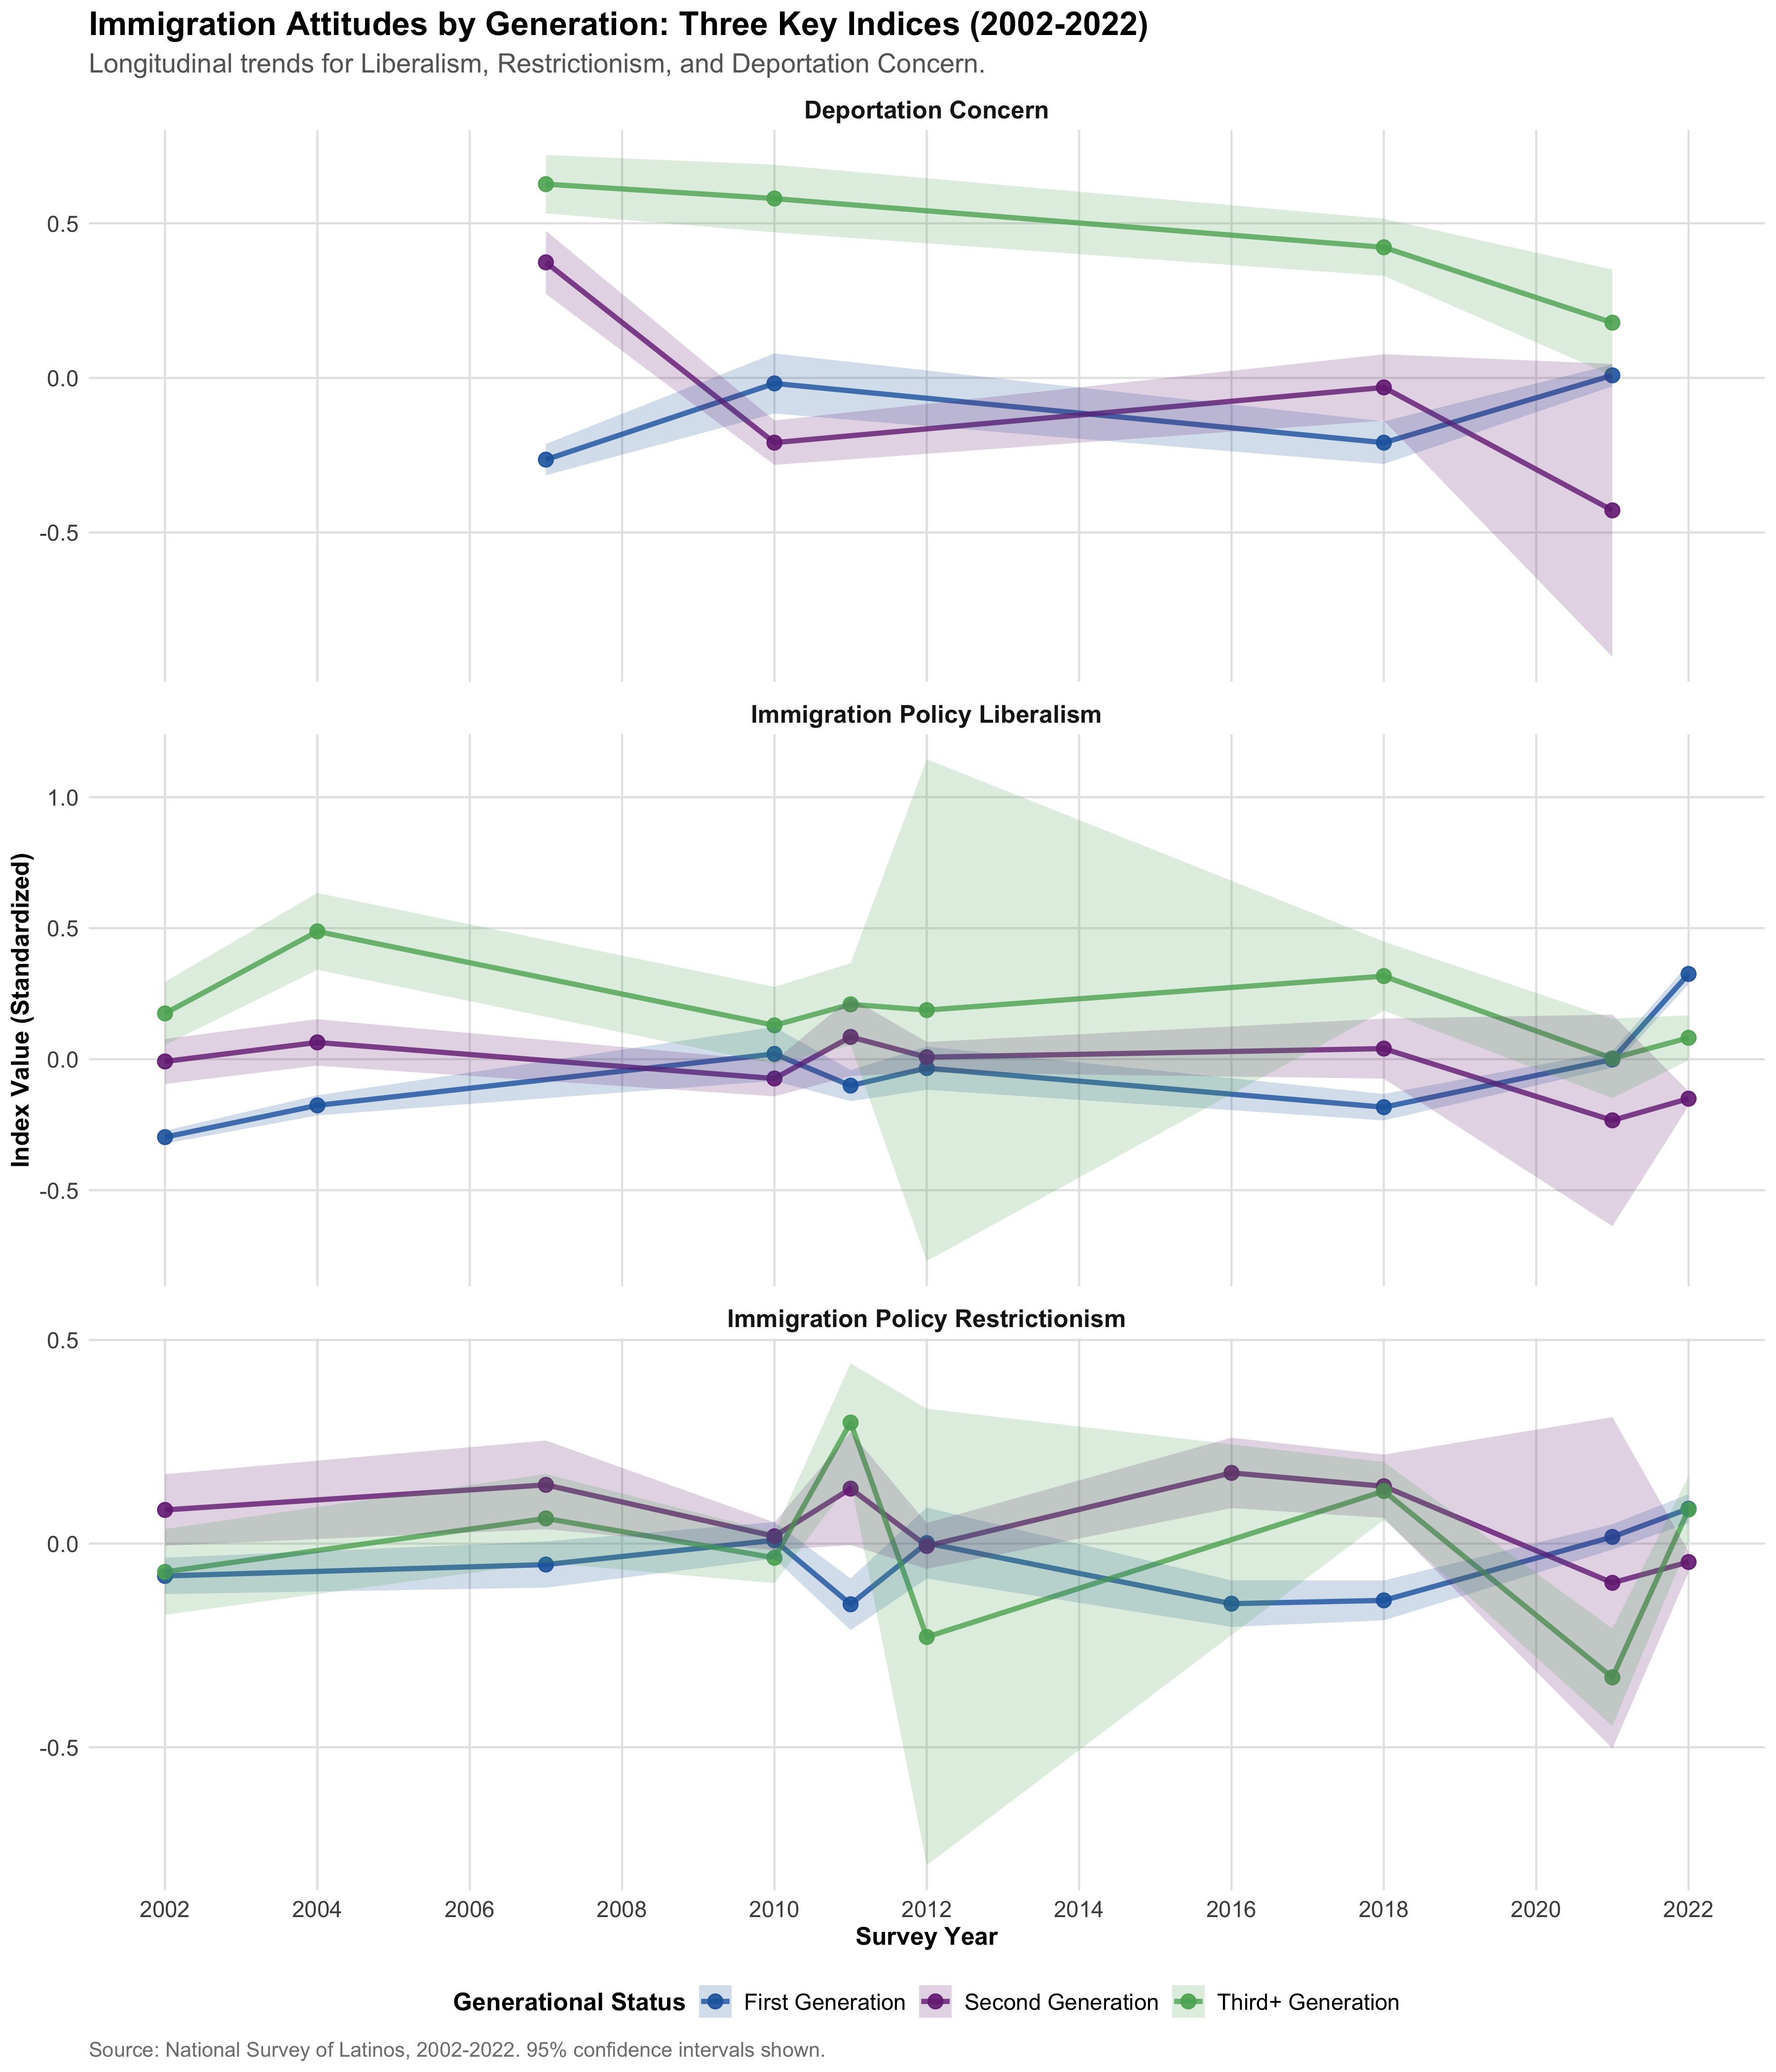
\includegraphics[width=0.95\textwidth]{../../outputs/CURRENT_2025_08_09_FIGURES_gold_standard/three_indices_by_generation_2002_2022.png}
    \caption{Immigration attitudes by generation across three key indices, showing distinct generational patterns over the 20-year study period.}
    \label{fig:three_indices}
\end{figure}

\subsection{Generational Coding}
\begin{itemize}
    \compactdesc{1st Gen}{Foreign-born}
    \compactdesc{2nd Gen}{U.S.-born, at least one foreign-born parent}
    \compactdesc{3rd+ Gen}{U.S.-born, U.S.-born parents}
\end{itemize}

\section{Findings}

\subsection{The Illusion of Stability}

Across the total Hispanic population, aggregate attitudes on immigration appear relatively stable over 20 years. However, \textbf{this stability masks significant and diverging trends between immigrant generations.}

\subsection{Generational Divergence: The 2021-2022 Role Reversal}

\textbf{Key Finding:} By 2022, first-generation immigrants had become more liberal than second-generation Hispanics -- a complete reversal from 2002 patterns.

\textbf{Statistical Evidence (NOFE Analysis):}

\begin{enumerate}
    \item \textbf{First Generation:}
        \begin{itemize}
            \item Liberalism: +0.020 per year (p=0.019*)
            \item Pattern: Steady liberalization accelerating post-2020
            \item 2002: -0.30 (most restrictionist) $\rightarrow$ 2022: +0.33 (most liberal)
            \item Mechanism: \textbf{Reactive integration} -- policy threats strengthen pro-immigration attitudes
        \end{itemize}

    \item \textbf{Second Generation:}
        \begin{itemize}
            \item Liberalism: -0.010 per year (p=0.009**)
            \item Pattern: Becoming more restrictionist over time
            \item 2021-2022: Sharp restrictionist turn (-0.23 to -0.15)
            \item Mechanism: \textbf{Strategic distancing} from immigrant identity
        \end{itemize}

    \item \textbf{Third+ Generation:}
        \begin{itemize}
            \item Liberalism: -0.010 per year (p=0.191, ns)
            \item Pattern: Stable liberal baseline with minimal change
            \item Consistent positioning around +0.22 mean liberalism
            \item Mechanism: \textbf{Settled Americanism} -- stable attitudes typical of established populations
        \end{itemize}
\end{enumerate}

\begin{figure}[H]
    \centering
    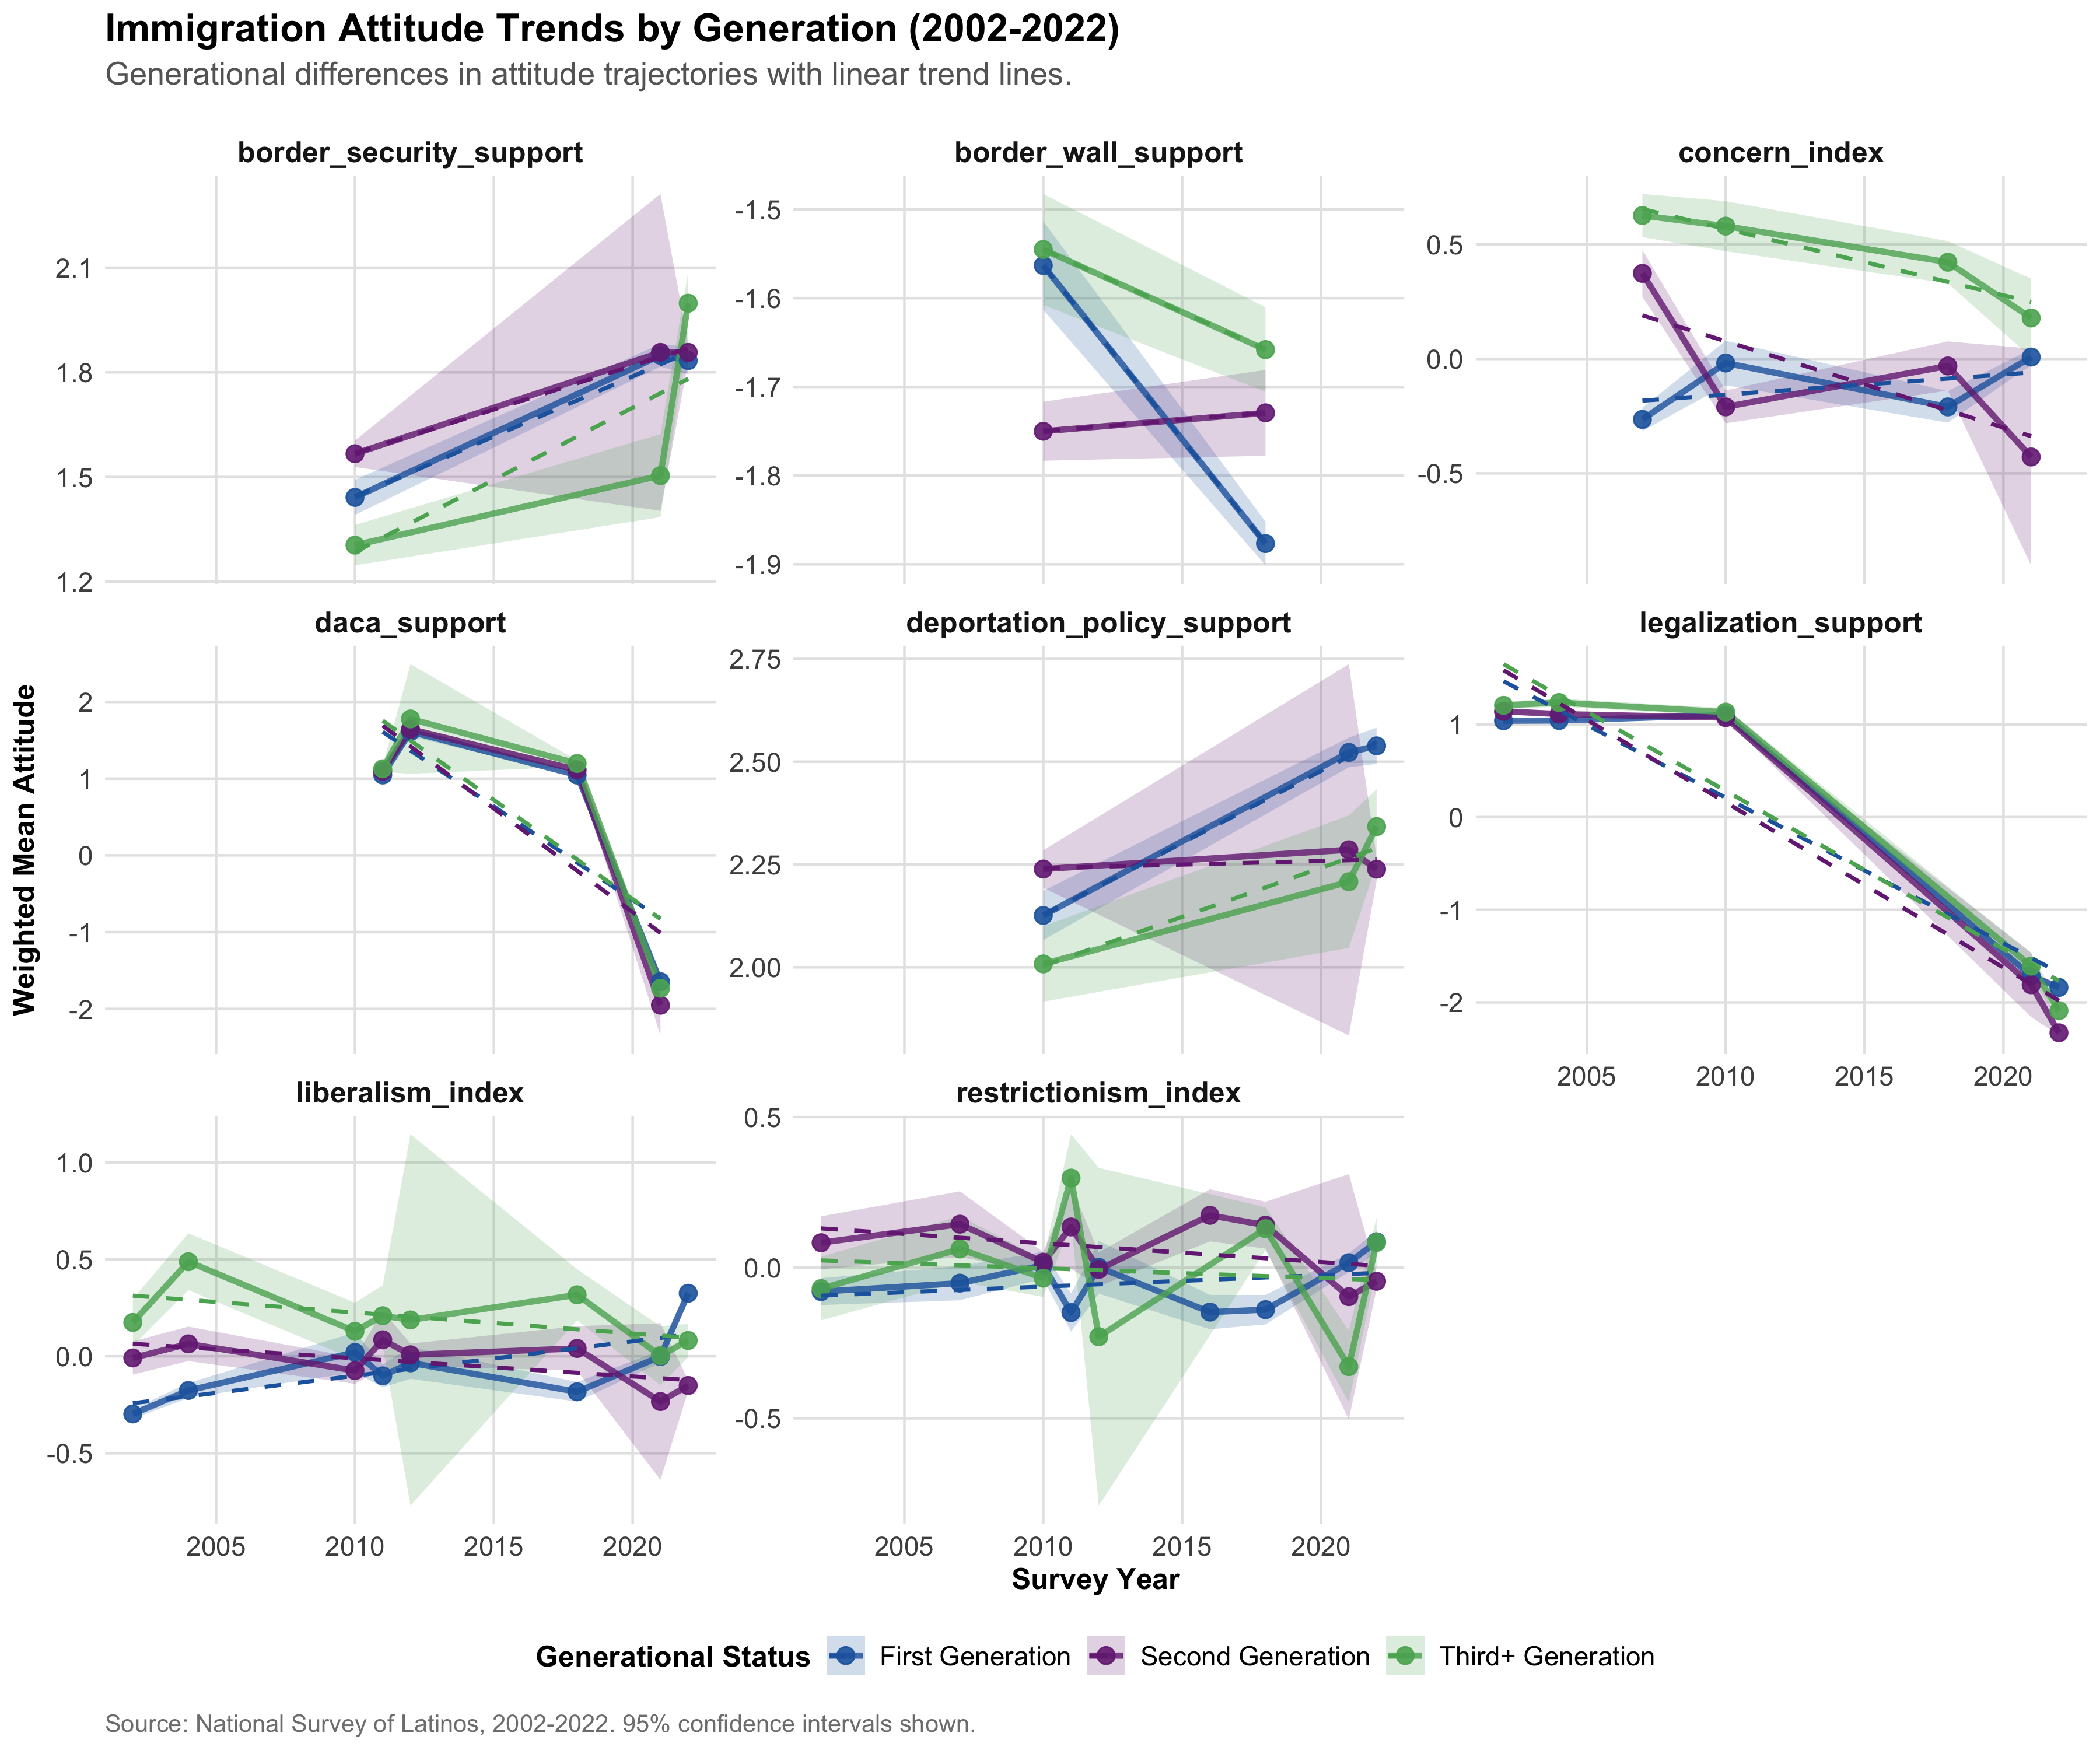
\includegraphics[width=0.9\textwidth]{../../outputs/CURRENT_2025_08_09_FIGURES_gold_standard/generation_trends_2002_2022.png}
    \caption{Generation-specific immigration attitude trends revealing distinct trajectories that challenge linear assimilation models.}
    \label{fig:generation_trends}
\end{figure}

\subsection{Critical Temporal Inflection Points}

Our fine-grained analysis identifies three critical moments:

\begin{enumerate}
    \item \textbf{2011: Obama Deportation Peak}
        \begin{itemize}
            \item Maximum generational divergence across all measures
            \item Peak deportation enforcement (400,000+ annual)
            \item Each generation adopts distinct defensive positioning
        \end{itemize}
        
    \item \textbf{2016: Pre-Trump Anticipatory Effects}
        \begin{itemize}
            \item Largest first-second generation gap (-0.32 difference)
            \item Attitude shifts precede actual policy implementation
            \item Evidence of political environment effects on attitudes
        \end{itemize}
        
    \item \textbf{2021-2022: Post-Trump Consolidation}
        \begin{itemize}
            \item First generation: Massive liberalization (+0.33 shift)
            \item Second generation: Sustained restrictionist positioning
            \item Complete role reversal in generational ordering
        \end{itemize}
\end{enumerate}

\subsection{Legalization Support: Question Format Change but Continued Support}

\textbf{2002-2010:} Direct support/oppose question shows overwhelming support:
\begin{itemize}
    \compactdesc{First Generation}{90-96\% support legalization}
    \compactdesc{Second Generation}{86-93\% support}
    \compactdesc{Third+ Generation}{76-87\% support}
\end{itemize}

\textbf{2021-2022:} New importance scale (treating ``very/somewhat important'' as support):
\begin{itemize}
    \compactdesc{First Generation}{80\% consider legalization important (moderate decline)}
    \compactdesc{Second Generation}{73\% consider important (notable decline)}
    \compactdesc{Third+ Generation}{80\% consider important (stable)}
\end{itemize}

\textbf{Key Finding:} Support remains substantial across all generations, though second generation shows the largest decline (-17 percentage points per decade).

\subsection{Volatility and Within-Generation Heterogeneity}

\textbf{Attitude Stability Analysis:}
\begin{itemize}
    \compactdesc{First Generation}{Highest liberalism volatility (CV = 3.35) -- most policy-responsive}
    \compactdesc{Second Generation}{Moderate volatility (CV = 3.31) -- strategic positioning}
    \compactdesc{Third+ Generation}{Stable liberalism (CV = 0.75) but extreme restrictionism volatility (CV = 17.8)}
\end{itemize}

\textbf{Within-Generation Distribution:}
\begin{itemize}
    \compactdesc{Third+ Generation}{Most heterogeneous (SD = 1.21) -- spans full political spectrum}
    \compactdesc{First Generation}{Most homogeneous (SD = 0.84) -- shared immigrant experience}
\end{itemize}

\section{Central Argument: Multi-Track Generational Response Model}

The phenomenon of ``immigrants against immigrants'' reflects three distinct generational response mechanisms to the U.S. immigration policy environment, challenging traditional linear assimilation models.

\subsection{Three Generational Tracks}

\subsubsection{Track 1: Reactive Integration (1st Generation)}
\begin{itemize}
    \item Integration experiences lead to increased pro-immigration attitudes
    \item Policy threats trigger delayed but intense liberal mobilization
    \item 2-3 year lag in response to policy changes
    \item Highest volatility reflects active policy monitoring
\end{itemize}

\subsubsection{Track 2: Strategic Distancing (2nd Generation)}
\begin{itemize}
    \item Status anxiety drives differentiation from immigrant identity
    \item Immediate, counter-cyclical responses to first generation
    \item When immigration becomes salient, adopt restrictionist positions
    \item Fastest decline in legalization support signals active distancing
\end{itemize}

\subsubsection{Track 3: Settled Americanism (3rd+ Generation)}
\begin{itemize}
    \item Stable American identity with consistent liberal baseline
    \item Minimal policy responsiveness
    \item Attitudes reflect mainstream American political divisions
    \item Bipolar pattern: stable liberalism but volatile restrictionism
\end{itemize}

\subsection{Reconciling Electoral vs. Attitudinal Data}

Media narratives of ``Latino rightward shift'' capture real electoral changes but miss the complex attitudinal dynamics underneath.

\begin{itemize}
    \compactdesc{Electoral Evidence}{Trump gained 8+ percentage points among Latinos (2016→2020)}
    \compactdesc{Attitude Reality}{First generation actually becoming more liberal}
    \compactdesc{Resolution}{Electoral shifts driven by turnout, geography, and second-generation volatility}
    \compactdesc{Key Insight}{Short electoral cycles miss long-term generational divergence}
\end{itemize}

\subsection{Mechanisms Driving the Patterns}

\begin{enumerate}
    \item \textbf{Political Learning:} Immigrants learn American political contradictions
    \item \textbf{Identity Complexity:} Multiple identities create cross-pressures
    \item \textbf{Policy Environment:} External threats shape group consciousness
    \item \textbf{Generational Positioning:} Each generation finds distinct political space
\end{enumerate}

\section{Implications}

\subsection{For Theory}

\begin{enumerate}
    \item \textbf{Non-Linear Assimilation:} Challenges to straight-line models are confirmed
        \begin{itemize}
            \item Generations don't progress linearly toward ``American'' attitudes
            \item Multiple pathways exist, consistent with segmented assimilation
            \item Context and timing matter more than generational distance
        \end{itemize}
    
    \item \textbf{Reactive Ethnicity:} Strong support for policy-driven identity formation
        \begin{itemize}
            \item First generation mobilizes during threat periods
            \item Identity becomes more salient under restrictionist policies
        \end{itemize}
    
    \item \textbf{Multidimensional Attitudes:} Immigration attitudes aren't unidimensional
        \begin{itemize}
            \item Liberalism and restrictionism can coexist
            \item Different policy domains elicit different responses
        \end{itemize}
\end{enumerate}

\subsection{For Politics \& Policy}

\begin{enumerate}
    \item \textbf{Coalition Instability:} Generational divergence threatens Latino political unity
        \begin{itemize}
            \item Cannot assume uniform Latino positions on immigration
            \item Generation-specific messaging strategies required
            \item Long-term demographic change will shift political baselines
        \end{itemize}
    
    \item \textbf{Policy Design:} Different frames for different generations
        \begin{itemize}
            \item First generation: Integration success, anti-discrimination
            \item Second generation: Avoid explicit immigrant framing
            \item Third+ generation: Standard liberal humanitarian appeals
        \end{itemize}
        
    \item \textbf{Temporal Effects:} Policy announcements create anticipatory positioning
        \begin{itemize}
            \item Attitudes shift before policy implementation
            \item First generation shows 2-3 year delayed responses
            \item Electoral cycles miss longer-term attitude evolution
        \end{itemize}
\end{enumerate}

\section{Conclusion}

\subsection{Central Finding}
``Immigrants against immigrants'' reflects complex generational response patterns to the U.S. political environment, not simple hypocrisy or linear assimilation. The 2021-2022 role reversal -- where first-generation immigrants became more liberal than their American-born children -- represents a significant challenge to traditional assimilation theories.

\subsection{Methodological Contributions}
\begin{itemize}
    \item Multi-index measurement captures attitude complexity
    \item Fine-grained temporal analysis reveals critical inflection points
    \item NOFE approach successfully identifies linear trends
    \item 20-year scope captures multiple policy cycles
\end{itemize}

\subsection{Theoretical Advancement}
This research contributes to immigration scholarship by:
\begin{itemize}
    \item Documenting non-linear assimilation patterns
    \item Identifying three distinct generational response mechanisms
    \item Showing how policy environments shape attitude formation
    \item Demonstrating the importance of temporal analysis
\end{itemize}

\subsection{Future Directions}
\begin{enumerate}
    \item Investigate the legalization support collapse (measurement artifact?)
    \item Test generational mechanisms through survey experiments
    \item Compare Latino patterns to other immigrant groups
    \item Examine geographic and origin-country variation
    \item Link attitude patterns to actual voting behavior
\end{enumerate}

\section{Technical Appendix}

\subsection{Data Quality Standards}
\begin{itemize}
    \compactdesc{Temporal Coverage}{20 years across 4 presidential administrations}
    \compactdesc{Sample Size}{30,869 observations with valid generation labels}
    \compactdesc{Methodology}{Pew Research Center's rigorous sampling}
    \compactdesc{Statistical Approach}{Weighted OLS without fixed effects (NOFE)}
    \compactdesc{Coverage Rates}{Core indices 59-63\%, adequate for robust inference}
    \compactdesc{Robustness}{Multiple measures confirm generational patterns}
\end{itemize}

\subsection{Analysis Scripts}
\begin{itemize}
    \item Fine-Grained Analysis: \texttt{CURRENT\_2025\_08\_09\_ANALYSIS\_fine\_grained\_patterns.R}
    \item Gold Standard Visuals: \texttt{CURRENT\_2025\_08\_09\_UPDATE\_gold\_standard\_visuals.R}
    \item Three Indices Analysis: \texttt{CURRENT\_2025\_08\_09\_ANALYSIS\_three\_indices\_plot.R}
    \item Bug-Fixed Scripts: See \texttt{CURRENT\_2025\_08\_09\_BUG\_FIX\_REPORT.md}
\end{itemize}

\vspace{1em}
\noindent\rule{\textwidth}{0.2pt}

\begin{center}
\textbf{Analysis Version:} Gold Standard 2025.08.09 | \textbf{Date:} August 2025
\end{center}

\end{document}
